% DO NOT COMPILE THIS FILE DIRECTLY!
% This is included by the other .tex files.

\begin{frame}[t,plain]
\titlepage
\end{frame}




\begin{frame}[t]{Decompilación}

\textbf{Uso de Apktool}

\begin{wrapfigure}{r}{0.43\textwidth} 
\vspace{2pt}
  \begin{center}
    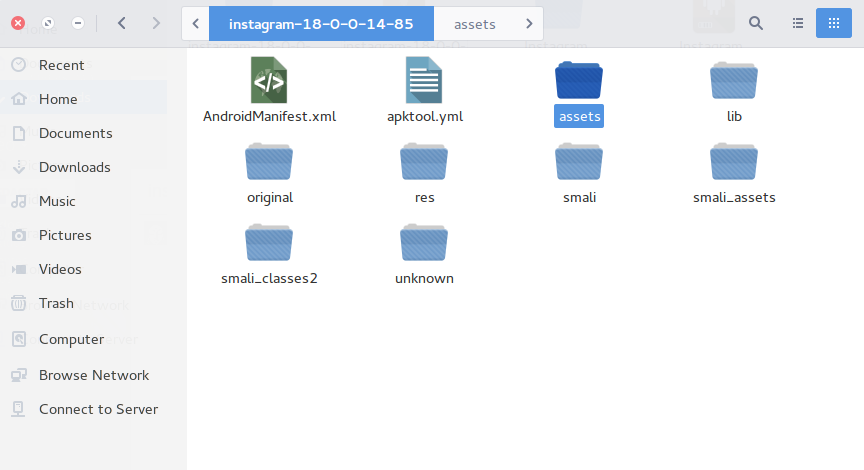
\includegraphics[width=0.45\textwidth]{apktool.png}
    \label{fig:databaseUserTable}
  \end{center}
  \vspace{2pt}
\end{wrapfigure} 

\bigskip

Uso de herramienta \textbf{apktool} 
\begin{center}
    apktool d Instagram.apk
\end{center}
 \\
 
 se obtendrá archivos correspondientes a la aplicación además de los layouts, res y clasess especificas del mismo.

\end{frame}

\begin{frame}[t,fragile]{Decompilación}

\textbf{Obtención de XML}

\begin{wrapfigure}{r}{0.43\textwidth} 
\vspace{2pt}
  \begin{center}
    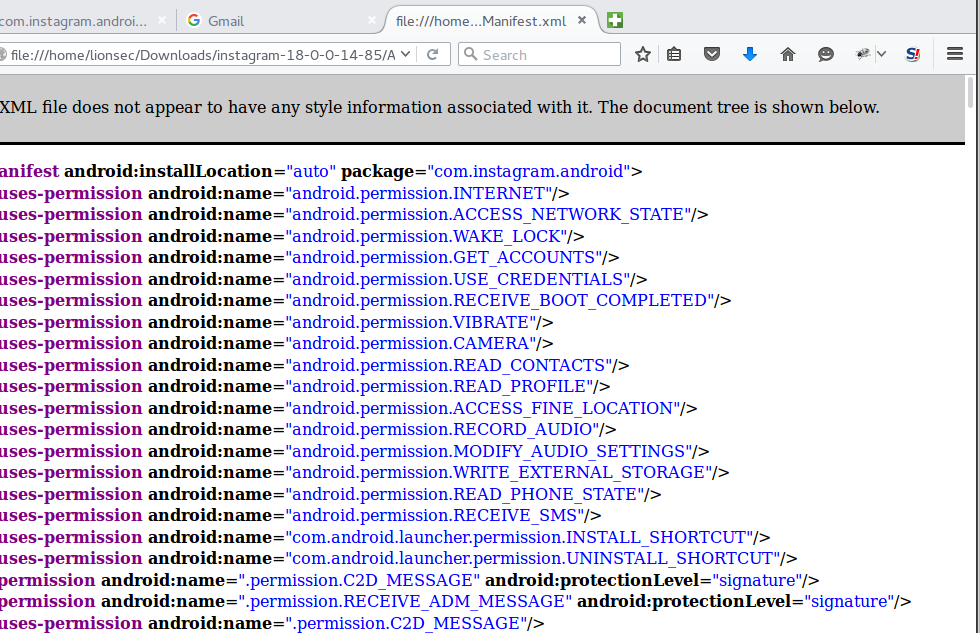
\includegraphics[width=0.45\textwidth]{xml.png}
    \label{fig:databaseUserTable}
  \end{center}
  \vspace{2pt}
\end{wrapfigure} 

\bigskip

 Por medio de la herrramienta \textbf{apktool} y utilizando consola. se aplica comando
\begin{center}
    apktool d Instagram.apk
\end{center}
 \\
 
 se obtendrá los xml y archivos correspondientes a la aplicación.

\end{frame}

\begin{frame}[t,fragile]{Decompilación}

\textbf{Obtención de Java}

\begin{wrapfigure}{r}{0.43\textwidth} 
\vspace{2pt}
  \begin{center}
    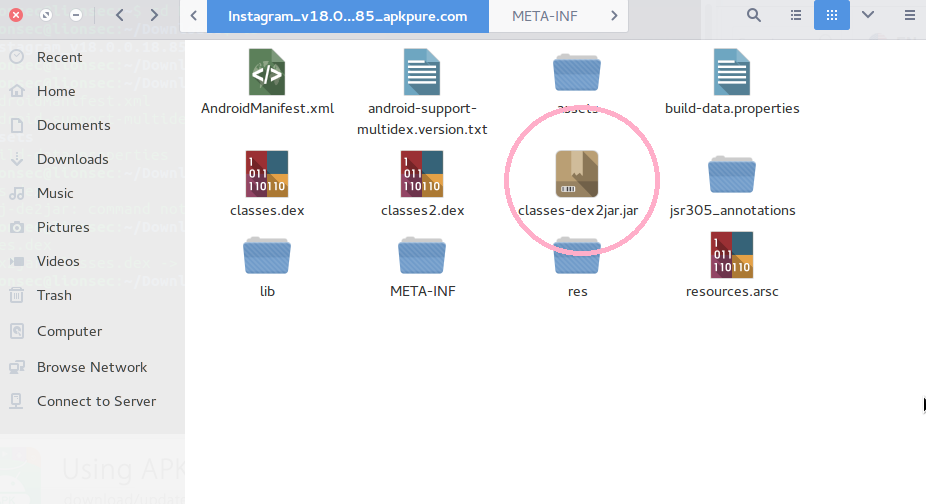
\includegraphics[width=0.45\textwidth]{jarclases.png}
    \label{fig:databaseUserTable}
  \end{center}
  \vspace{2pt}
\end{wrapfigure} 

\bigskip

 Por medio de la herramienta \textbf{dex2jar} y utilizando consola. se aplica comando
\begin{center}
    d2j-dex2jar classes.dex
\end{center}
 \\
 
 se utiliza el dex (Dalvik Executable) para obtener el comprimido del archivo APK. Lo que puede ser visto con un java decompiler, accediendo entonces a el archivo.

\end{frame}


\begin{frame}[t,fragile]{Decompilación}

\textbf{Ver Archivos React}

\begin{wrapfigure}{r}{0.43\textwidth} 
\vspace{2pt}
  \begin{center}
    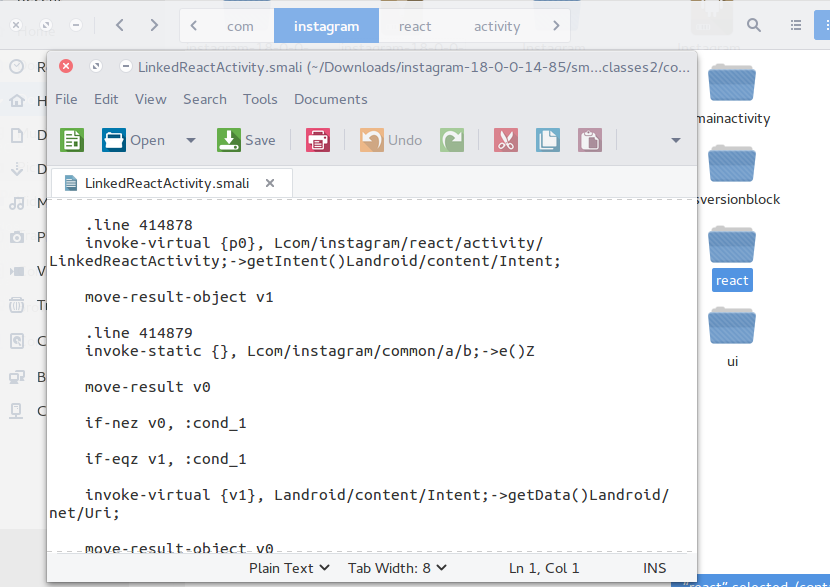
\includegraphics[width=0.45\textwidth]{react.png}
    \label{fig:databaseUserTable}
  \end{center}
  \vspace{2pt}
\end{wrapfigure} 

\bigskip

 Se encuentran los archivos de react correspondiente las actividades, delegados o bien los archivos \textbf{.smali} correspondientes al assembly de lenguaje Java.

\end{frame}

\begin{frame}[t,fragile]{Decompilación}

\textbf{Hosts}

\begin{wrapfigure}{r}{0.43\textwidth} 
\vspace{2pt}
  \begin{center}
    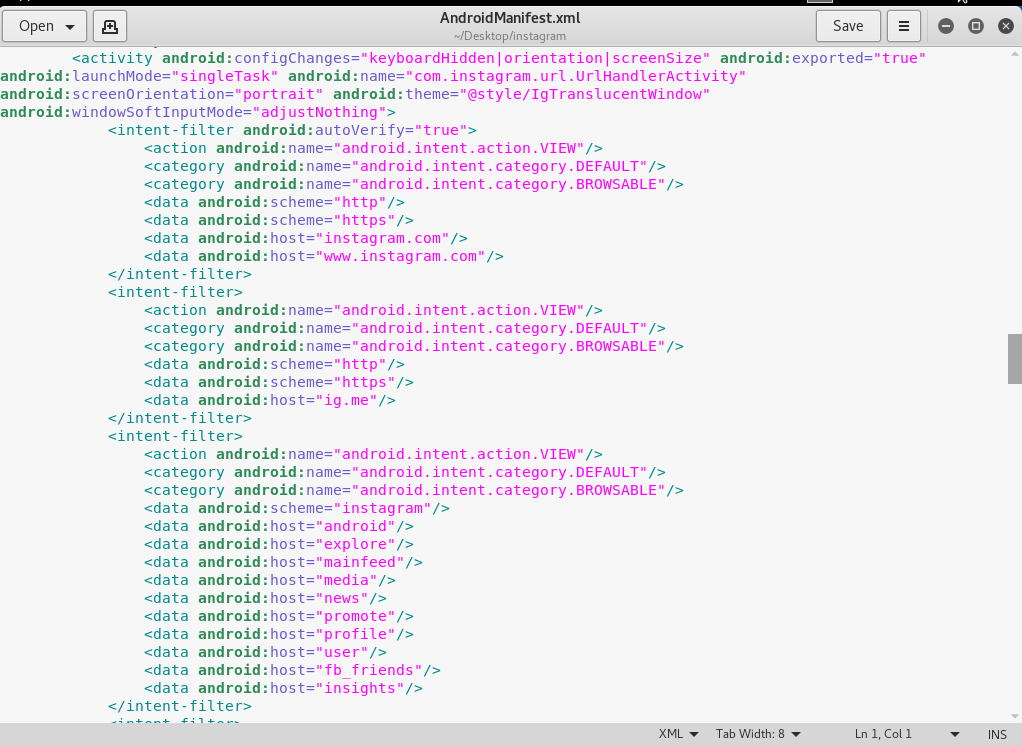
\includegraphics[width=0.45\textwidth]{xmlhost.png}
    \label{fig:databaseUserTable}
  \end{center}
  \vspace{2pt}
\end{wrapfigure} 

\bigskip

En la siguiente figura se logra apreciar el Host principal correspondiente a la aplicación, dando a entender que :

\begin{center}
    www.instagram.com    
\end{center}
será la url, host del resto de actividades.



\end{frame}

\begin{frame}[t,fragile]{Host a Probar}

\textbf{Hosts Encontrados en AndroidManifest.xml}

\begin{wrapfigure}{r}{0.43\textwidth} 
\vspace{2pt}
  \begin{center}
    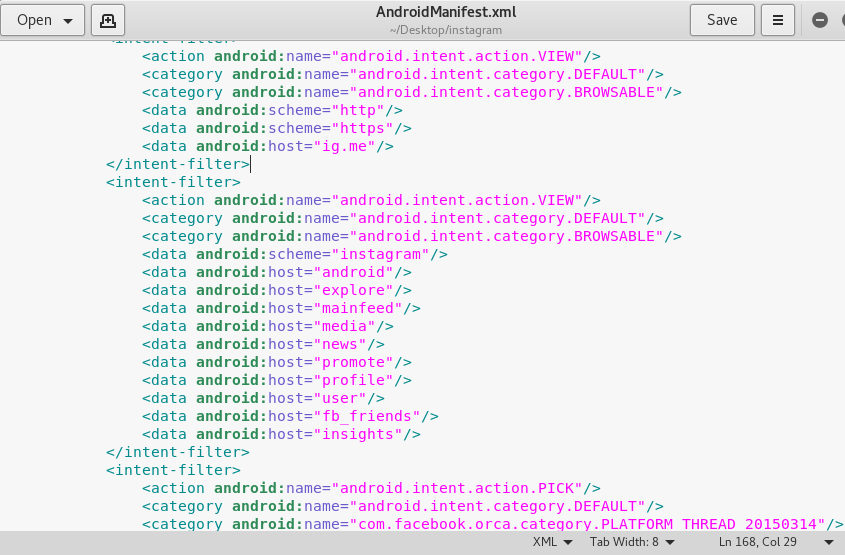
\includegraphics[width=0.45\textwidth]{xmlhostbrowser.png}
    \label{fig:databaseUserTable}
  \end{center}
  \vspace{2pt}
\end{wrapfigure} 

\bigskip

Una vez conocida la url, se procede por medio de sqlmap a analizar el siguiente listado de host (Browsers) respectivos a la api:


\begin{itemize}
\item android
\item explore
\item mainfeed
\item media
\item news
\item entre otros.
\end{itemize}

\end{frame}

\begin{frame}[t,fragile]{Herramientas}

\textbf{Uso de SQLMAP}

\begin{wrapfigure}{r}{0.43\textwidth} 
\vspace{2pt}
  \begin{center}
    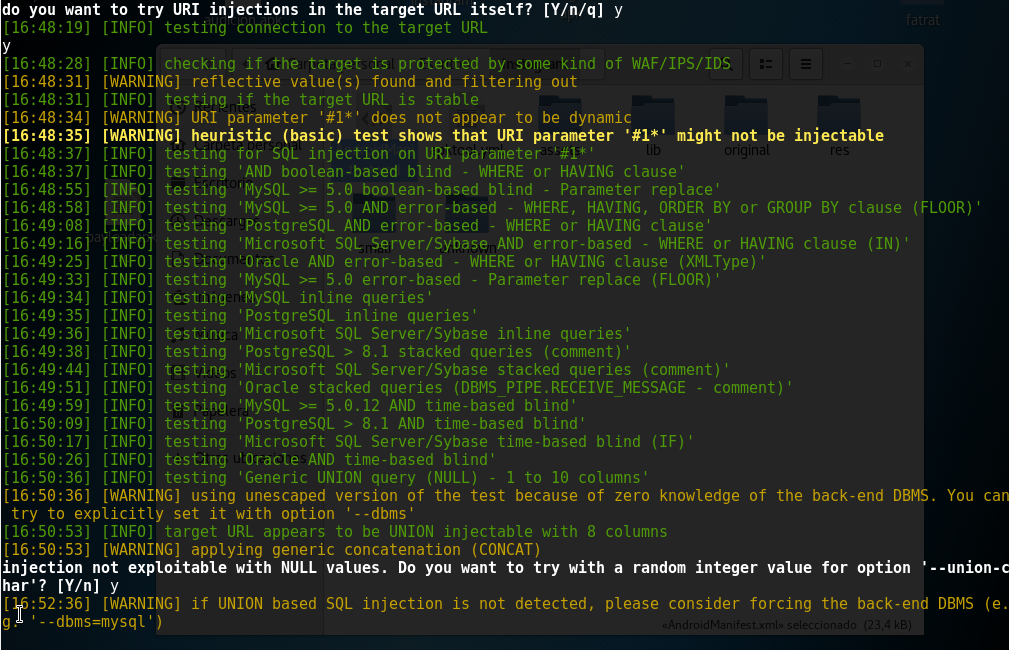
\includegraphics[width=0.45\textwidth]{testsqlmap.png}
    \label{fig:databaseUserTable}
  \end{center}
  \vspace{2pt}
\end{wrapfigure} 

\bigskip

 Tras utilizar el comando:
 
 \begin{center}
     sqlmap -u www.instagram.com/ Host Browsers 
 \end{center}
 
 Realizando inyecciones dentro de la aplicación, de tal manera que se busquen fugas o posibles consultas. 

\end{frame}


\begin{frame}[t,fragile]{Herramientas}

\textbf{Uso de SQLMAP}

\begin{wrapfigure}{r}{0.43\textwidth} 
\vspace{2pt}
  \begin{center}
    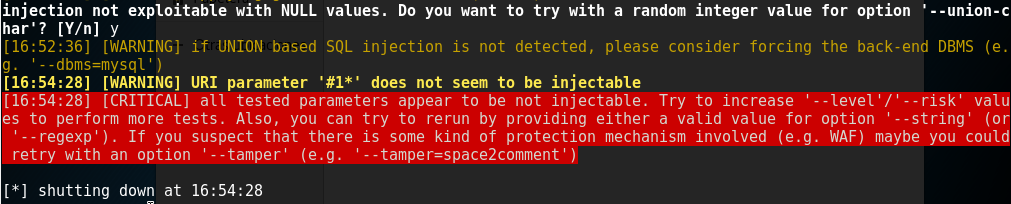
\includegraphics[width=0.45\textwidth]{errortest.png}
    \label{fig:databaseUserTable}
  \end{center}
  \vspace{2pt}
\end{wrapfigure} 

\bigskip

 Encontrando el siguiente error, lo que implica que no se logró hacer ninguna inyección exitosa dentro de la aplicación.

\end{frame}

\begin{frame}[t,fragile]{Herramientas}

\textbf{Uso de NMAP}

\begin{wrapfigure}{r}{0.43\textwidth} 
\vspace{2pt}
  \begin{center}
    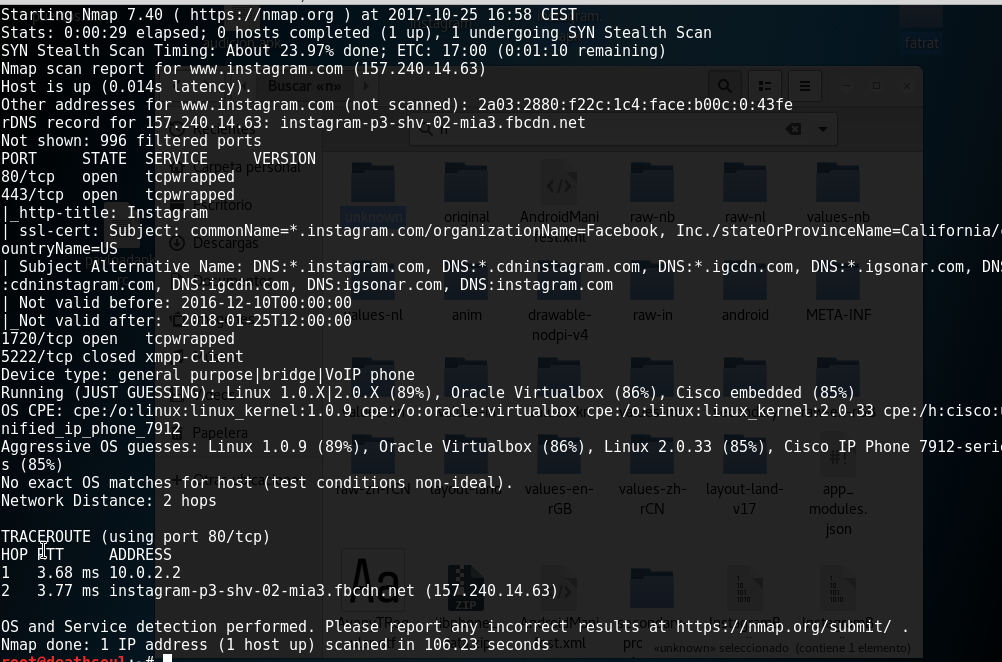
\includegraphics[width=0.45\textwidth]{nmap.png}
    \label{fig:databaseUserTable}
  \end{center}
  \vspace{2pt}
\end{wrapfigure} 

\bigskip

 Tras utilizar el comando:
 
 \begin{center}
     nmap -O www.instagram.com 
 \end{center}
 
Obteniendo los puertos abiertos dentro de la aplicación:

\begin{itemize}
    \item Puerto 80/tcp
    \item Puerto 443/tcp
\end{itemize}

\end{frame}

\begin{frame}[t,fragile]{Herramientas}

\textbf{Uso de Wireshark}

\begin{wrapfigure}{r}{0.43\textwidth} 
\vspace{2pt}
  \begin{center}
    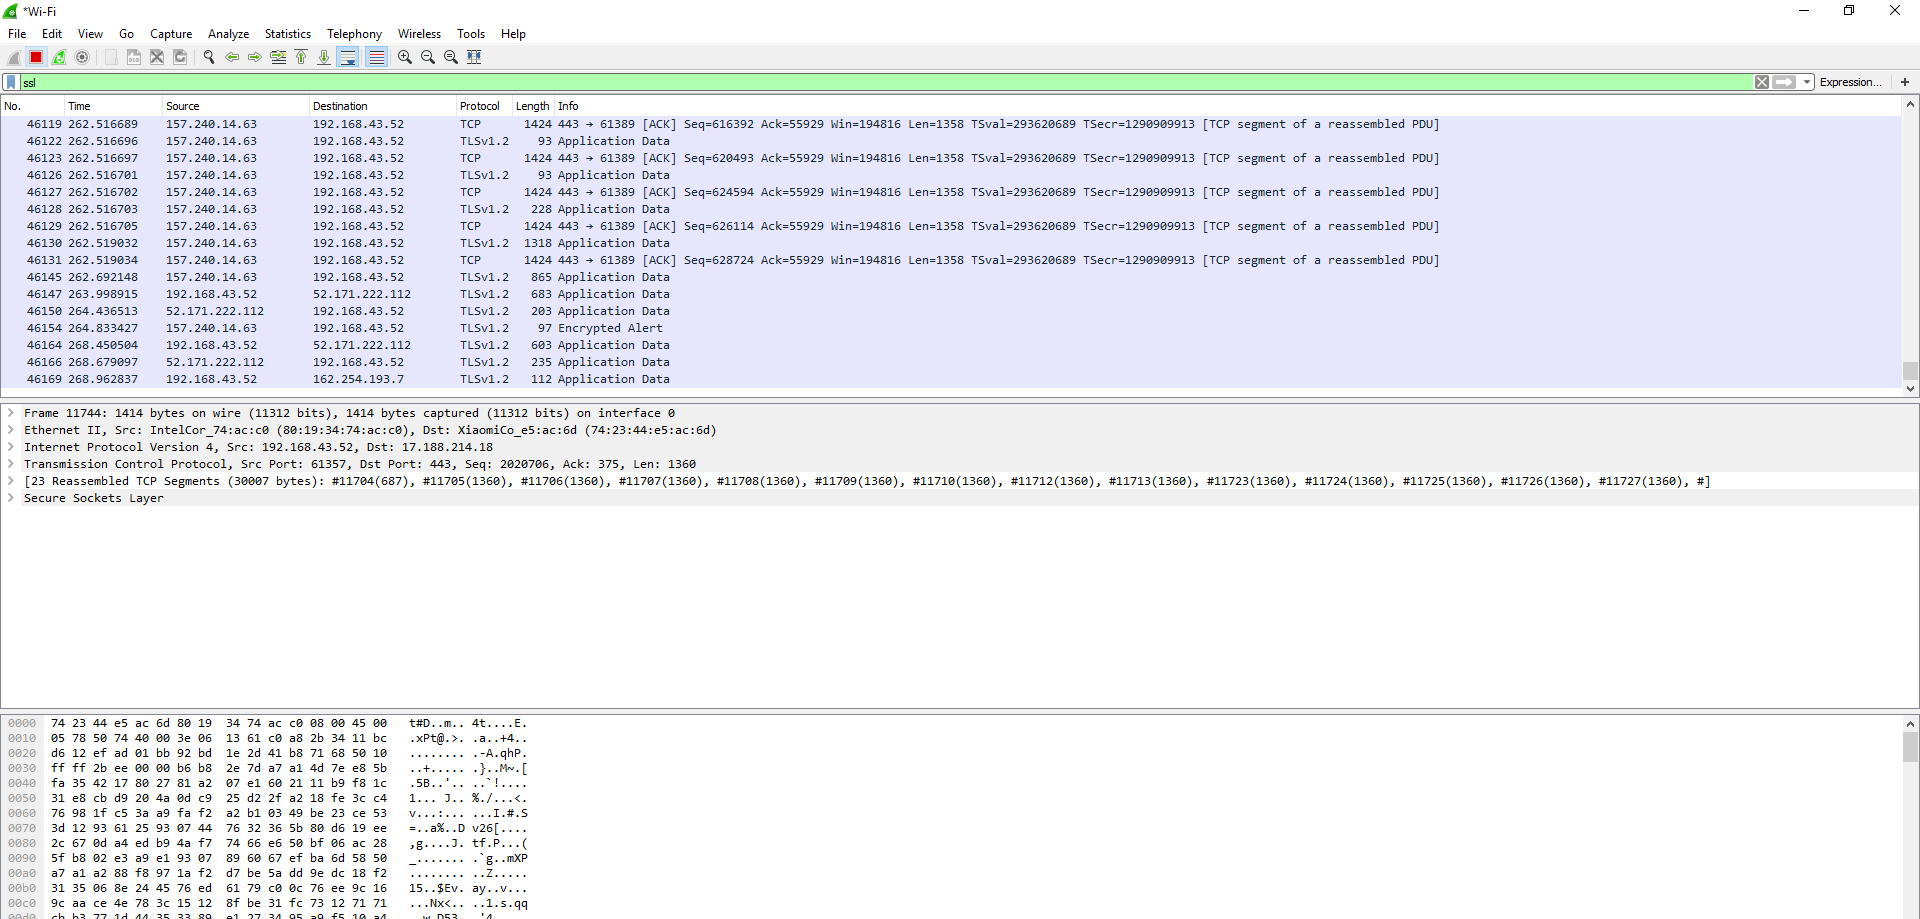
\includegraphics[width=0.45\textwidth]{wireshark.png}
    \label{fig:databaseUserTable}
  \end{center}
  \vspace{2pt}
\end{wrapfigure} 

\bigskip

Mediante el uso de wireshark, se realizan análisis de los paquetes captados en conjunto con la aplicación, de las cuales no se logra encontrar paquetes expuestos. 

\end{frame}